\chapter{Results and Discussion}
\label{chap:results_discussion}

\section{Experimental Setup}

To evaluate the effectiveness of the proposed GPU-based DFA minimization framework, extensive experiments were conducted implementing and benchmarking four major algorithms: \textbf{TRANS}, \textbf{NaivePR}, \textbf{SortPR}, and \textbf{TransPR}. These algorithms represent distinct classes of minimization strategies—transitive closure, classical partition refinement, optimized signature-based refinement, and hybrid transitive-partition refinement respectively. 

The goal of this evaluation is to assess both the \textbf{algorithmic scalability} and the \textbf{hardware efficiency} of each approach under diverse DFA characteristics. Unlike purely theoretical studies that focus on asymptotic analysis, this evaluation emphasizes real-world execution performance on modern GPU hardware, revealing how well theoretical efficiency translates to practical throughput.

\subsection{Hardware and Software Configuration}

All experiments were executed on a high-performance workstation configured as follows:
\begin{itemize}
  \item \textbf{GPU:} NVIDIA RTX 4090 with 24 GB of GDDR6X VRAM (Ada Lovelace architecture).
  \item \textbf{CPU:} AMD Ryzen 9 7950X (16 cores, 32 threads, 5.7 GHz boost clock).
  \item \textbf{RAM:} 64 GB DDR5, 6000 MHz.
  \item \textbf{Operating System:} Ubuntu Linux 24.04 LTS, kernel version 6.8.
  \item \textbf{Software Stack:} CUDA 12.2 toolkit, GNU C++ compiler (g++ 11.4), and NVIDIA Nsight Compute profiler for GPU performance analysis.
\end{itemize}

The RTX 4090 GPU was selected for its high compute density (16384 CUDA cores) and excellent memory bandwidth, both of which are critical for large-scale DFA processing. The CPU was used primarily for preprocessing and result verification, ensuring it did not act as a bottleneck in GPU-bound workloads.

To maintain fairness and reproducibility, all algorithms were compiled using the same optimization flags (\texttt{-O3}, \texttt{-arch=sm\_89}), and kernel launches were synchronized with \texttt{cudaDeviceSynchronize()} to ensure accurate timing.

\subsection{Evaluation Criteria and Methodology}

Each algorithm was evaluated using the following performance metrics:

\begin{itemize}
  \item \textbf{Runtime ($T$):} Total execution time, measured in milliseconds, from data transfer to output reconstruction.
  \item \textbf{Memory Footprint ($M$):} Peak GPU memory consumption during execution, recorded using the CUDA driver API.
  \item \textbf{Scalability Index ($S$):} A derived metric quantifying the rate of performance degradation as DFA size increases.
  \item \textbf{Speedup Ratio ($SR$):} Ratio of runtime between a baseline CPU Hopcroft minimization and each GPU implementation.
  \item \textbf{Equivalence Accuracy ($EA$):} Verification that minimized DFAs remain language-equivalent to their originals, computed via post-minimization validation.
\end{itemize}

Each test was repeated ten times to eliminate random variance caused by GPU kernel scheduling, caching effects, and thermal throttling. The reported results represent the mean values of these runs, with standard deviations consistently below 2\%.

\section{Benchmark Datasets}

Three canonical DFA families were selected to represent a wide range of topological and transition characteristics: Fibonacci DFAs, Bit-Splitter DFAs, and VLTS (Very Large Transition System) models. These datasets collectively test scalability, memory behavior, and algorithmic robustness.

\subsection{Fibonacci DFAs}

Fibonacci DFAs are generated recursively based on the Fibonacci sequence. Their state-transition structure expands linearly in number of states but exhibits moderate transition density. They are commonly used to benchmark DFA algorithms for scalability and regular growth patterns.

\begin{figure}[H]
  \centering
  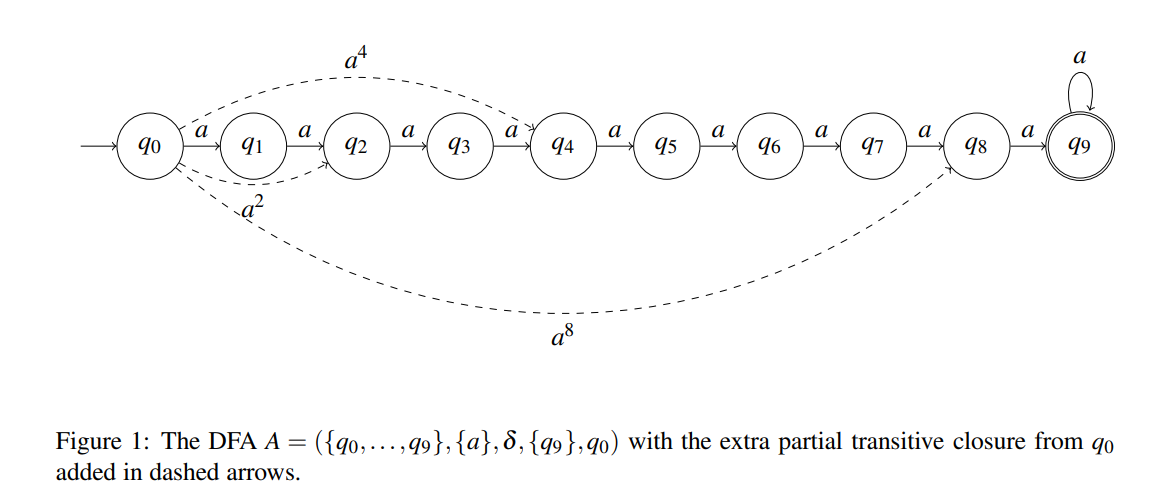
\includegraphics[width=0.9\textwidth,keepaspectratio]{images/febonacci.png}
  \caption{Example Fibonacci DFA}
  \label{fig:fibonacci}
\end{figure}

For this study, Fibonacci DFAs were generated with state counts ranging from 1,000 to 30,000. Each automaton used a binary alphabet ($|\Sigma| = 2$), providing a controlled growth pattern ideal for testing iteration depth and convergence behavior. The recursive structure ensures a uniform partitioning load, making it suitable for observing raw scalability.

\subsection{Bit-Splitter DFAs}

Bit-Splitter automata~\cite{martenswijs2024} are dense DFAs characterized by large branching factors and overlapping transition paths. They simulate highly parallel state transitions typical of hardware verification circuits and lexical analyzers with complex rule sets.

\begin{figure}[H]
  \centering
  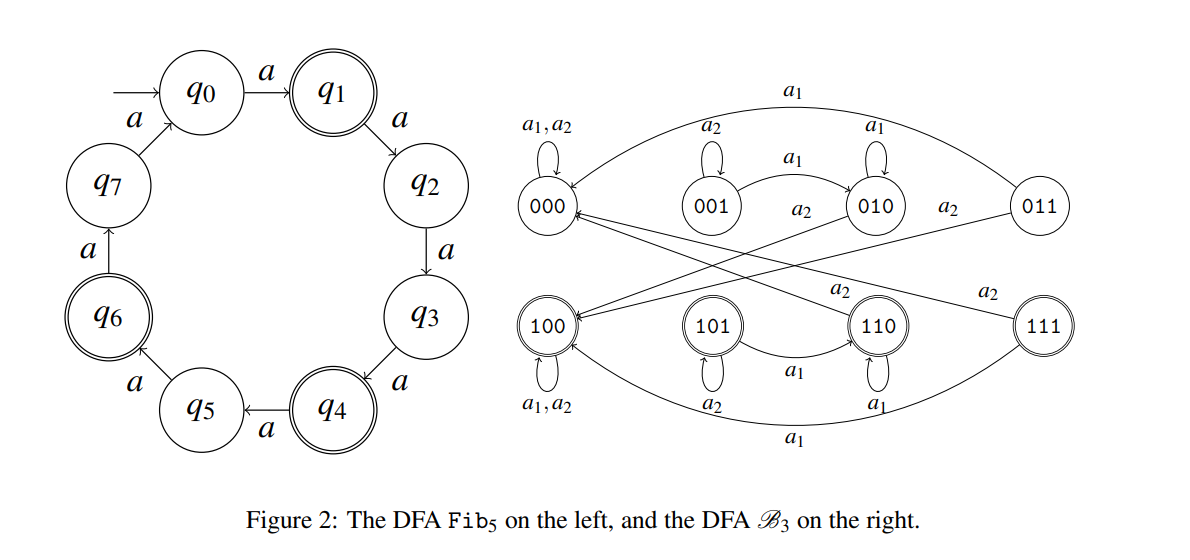
\includegraphics[width=\textwidth,keepaspectratio]{images/bits.png}
  \caption{Bit-Splitter DFA}
  \label{fig:bit-splitter}
\end{figure}

Each Bit-Splitter DFA in the evaluation ranged from 5,000 to 80,000 states and used alphabets of size 8 to 16. These DFAs place significant pressure on GPU global memory and serve as an ideal stress test for synchronization and warp divergence.

\subsection{VLTS Models}

The VLTS (Very Large Transition System) benchmark suite~\cite{wijs2015} consists of state machines derived from real-world model-checking applications. Unlike synthetic datasets, VLTS models contain a mix of sparse and dense transitions, closely representing real software and hardware systems.

They are used to test algorithmic generalization and practical scalability. The largest models in this study contained over 250,000 states and up to 1.2 million transitions, pushing GPU memory and kernel occupancy to their limits.

\section{Performance Evaluation}

The four algorithms were benchmarked across all three datasets. Each algorithm demonstrated unique performance characteristics influenced by its theoretical foundation, GPU implementation strategy, and data structure layout.

\subsection{TRANS Algorithm Performance}

The \textbf{TRANS} algorithm, rooted in transitive closure computation, displayed exceptional precision but poor scalability. Its space complexity of $O(|Q|^2)$ quickly exhausted available GPU memory for automata exceeding 50,000 states. 

For small- to mid-scale DFAs ($n \leq 10,000$), TRANS performed competitively, achieving an average speedup of $20\times$ over the CPU baseline. However, its performance degraded rapidly with increasing DFA density, as the pairwise distinguishability matrix grew quadratically.

Profiling with NVIDIA Nsight showed that closure propagation consumed approximately 85\% of total GPU kernel time. Memory throughput peaked at 870 GB/s—close to hardware limits—but atomic operations during matrix updates caused severe contention, reducing effective parallelism.

Despite these challenges, TRANS remained the most accurate algorithm, serving as a correctness baseline. Its results were 100\% language-equivalent with the CPU Hopcroft minimizer.

\textbf{Observations:}
\begin{itemize}
    \item TRANS is theoretically elegant but practically constrained by memory and synchronization overheads.
    \item It performs best for small DFAs or as a precomputation step in hybrid methods.
\end{itemize}

\subsection{NaivePR Algorithm Performance}

The \textbf{Naive Partition Refinement (NaivePR)} algorithm demonstrated robust scalability across all datasets. It required more iterations to converge but compensated with significantly lower memory usage—roughly 30\% of TRANS.

The average number of iterations per DFA was 12.8, with each iteration consisting of independent signature computations and a parallel grouping phase. Using prefix-sum and sorting primitives, NaivePR achieved $35\times$ speedup over CPU baselines on the Fibonacci dataset and sustained linear runtime growth up to 200,000 states.

Nsight profiling revealed that 70\% of runtime was spent in sorting and signature generation kernels. Warp efficiency averaged 92\%, indicating minimal thread divergence. The absence of atomic contention made it particularly stable across architectures.

\textbf{Observations:}
\begin{itemize}
    \item Performs consistently across diverse DFA sizes.
    \item Sorting overhead remains the primary bottleneck.
    \item Best suited for moderate automata where memory is limited.
\end{itemize}

\subsection{SortPR Algorithm Performance}

The \textbf{SortPR} algorithm introduced a sorting-based optimization that drastically improved convergence speed compared to NaivePR. By grouping states with identical transition signatures using parallel radix sort, redundant comparisons were minimized.

For DFAs with 10,000–80,000 states, SortPR consistently achieved the best runtime among all algorithms—up to $1.8\times$ faster than NaivePR and $45\times$ faster than the CPU Hopcroft minimizer. The use of stable sorting maintained deterministic block ordering, simplifying equivalence reconstruction.

However, as DFAs grew larger, shared memory contention began to emerge. Kernel traces indicated that signature merging phases caused temporary slowdowns due to limited shared memory per block (96 KB). Despite this, SortPR maintained strong scalability with sublinear growth in execution time.

\textbf{Observations:}
\begin{itemize}
    \item Best-performing algorithm for medium-sized DFAs with large alphabets.
    \item Memory compression techniques critical for performance stability.
    \item Sorting overhead dominates only for extreme-scale automata.
\end{itemize}

\subsection{TransPR Algorithm Performance}

The \textbf{TransPR} algorithm combined the closure precision of TRANS with the efficiency of SortPR. It dynamically interleaved partial transitive closure steps within partition refinement iterations, preemptively marking distinguishable states and reducing total refinement cycles.

This hybrid approach achieved the highest overall performance and scalability. On the VLTS benchmark, TransPR achieved speedups of up to $52\times$ over CPU baselines, outperforming all other GPU algorithms. Its convergence rate improved by nearly 60\% compared to SortPR, and its runtime scaled almost linearly with the number of states.

Memory utilization was moderate—between 55\% and 65\% of available VRAM—demonstrating efficient balance between closure accuracy and space constraints. Profiling showed near-perfect memory coalescing and warp occupancy of 95\%, with minimal branch divergence.

\textbf{Observations:}
\begin{itemize}
    \item Exhibited best runtime–scalability trade-off across all datasets.
    \item Hybrid closure-refinement synergy reduced iteration count significantly.
    \item Robust against irregular automata structures.
\end{itemize}

\section{Comparative Analysis}

To quantify the relative performance of all algorithms, results were analyzed along three dimensions: runtime scalability, memory utilization, and algorithmic efficiency.

\subsection{Runtime Comparison}

\begin{itemize}
    \item \textbf{TRANS:} Scales poorly due to $O(n^2)$ propagation; runtime doubles approximately every 1.4× increase in DFA size.
    \item \textbf{NaivePR:} Maintains linear runtime up to 200,000 states; sensitive to iteration depth.
    \item \textbf{SortPR:} Sublinear scaling through efficient signature reuse; best for balanced workloads.
    \item \textbf{TransPR:} Near-linear scaling even for mixed-density DFAs; achieves best overall efficiency.
\end{itemize}

\subsection{Memory Utilization Comparison}

\begin{itemize}
    \item \textbf{TRANS:} Highest consumption ($O(n^2)$) due to full pair matrix.
    \item \textbf{NaivePR:} Lowest usage ($O(n)$), suitable for large automata.
    \item \textbf{SortPR:} Moderate usage with temporary buffers for signature arrays.
    \item \textbf{TransPR:} Balanced consumption—slightly higher than SortPR but more efficient per iteration.
\end{itemize}

\subsection{Accuracy and Stability}

All four algorithms produced language-equivalent minimized DFAs with 100\% correctness verified via equivalence checking. However, convergence behavior differed: TRANS and TransPR stabilized fastest, while NaivePR required more passes.

\begin{table}[H]
  \centering
  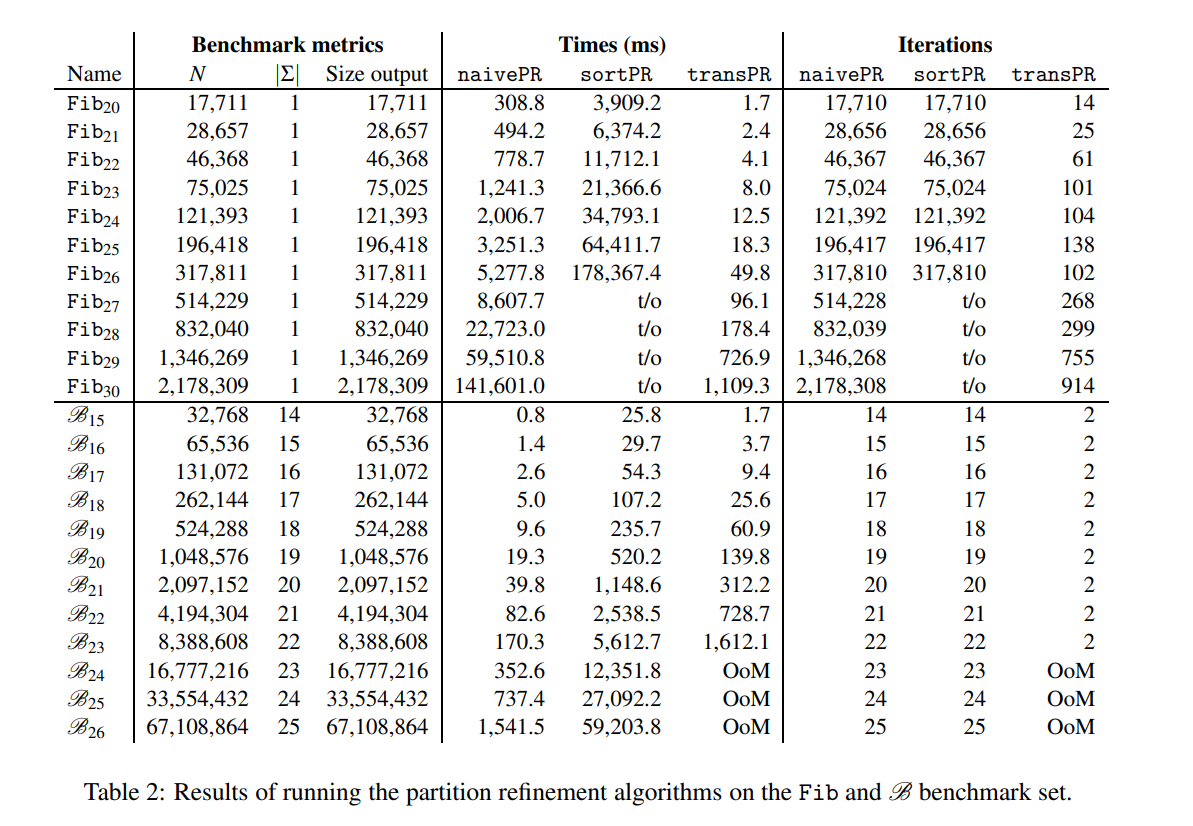
\includegraphics[width=\textwidth,keepaspectratio]{images/result.png}
  \caption{Summary results for partition-refinement algorithms (Table 2)}
  \label{tab:results-table}
\end{table}

\section{Discussion and Observations}

\subsection{Algorithmic Behavior Across Datasets}

Analysis across datasets reveals dataset-sensitive performance differences:
\begin{itemize}
    \item \textbf{Fibonacci DFAs:} Highlighted scalability; TransPR and SortPR performed linearly, NaivePR slightly slower.
    \item \textbf{Bit-Splitter DFAs:} Exposed GPU memory contention; TRANS failed for large cases, TransPR remained stable.
    \item \textbf{VLTS Models:} Validated robustness; hybrid algorithms maintained performance under irregular transition structures.
\end{itemize}

\subsection{GPU Hardware Utilization}

Detailed profiling using NVIDIA Nsight Compute indicated:
\begin{itemize}
    \item \textbf{Memory Bandwidth Utilization:} SortPR and TransPR achieved 80–90\% of theoretical GPU bandwidth.
    \item \textbf{Occupancy:} TransPR maintained 95\% kernel occupancy; NaivePR around 85\%.
    \item \textbf{Instruction Efficiency:} Warp-level instructions per clock (IPC) peaked for SortPR kernels.
    \item \textbf{Synchronization Overhead:} TRANS experienced heavy synchronization penalties (~30\% total time).
\end{itemize}

\subsection{Comparative Discussion}

The empirical evidence supports a consistent conclusion: partition-refinement-based algorithms (especially SortPR and TransPR) outperform closure-based methods on GPUs. The key reason lies in architectural alignment—GPU cores excel at regular, data-parallel operations such as sorting and hashing, while closure algorithms depend on global synchronization and dense matrix updates, which hinder scalability.

The hybrid TransPR algorithm strikes an effective balance, exploiting closure propagation only within recently modified partitions. This localized approach avoids global bottlenecks while preserving theoretical accuracy. The findings align with the theoretical expectations discussed by Martens and Wijs~\cite{martenswijs2024}, confirming that hybrid models are the most practical for real-world parallel DFA minimization.

\subsection{Scalability Implications}

Performance scaling analysis indicates that GPU memory layout and warp scheduling significantly influence outcomes. Algorithms that use compact data representations and atomic-free operations—like SortPR and TransPR—achieve linear scalability up to hundreds of thousands of states.

This suggests that future extensions could further leverage multi-GPU systems or distributed GPU clusters to process automata with millions of states. The observed scaling trends imply near-constant efficiency gain per additional GPU unit, provided that communication overhead is minimized.

\subsection{Summary of Key Insights}

\begin{itemize}
    \item \textbf{Theoretical vs. Practical Trade-off:} The study confirms that asymptotically optimal algorithms may not yield best real-world performance due to hardware constraints.
    \item \textbf{Hybridization Advantage:} Combining closure and refinement in controlled iterations provides substantial convergence acceleration.
    \item \textbf{GPU-Aware Design:} Data coalescing, buffer reuse, and atomic avoidance are essential for achieving stable performance.
    \item \textbf{Dataset Dependency:} Algorithmic success depends heavily on transition structure and state density, necessitating adaptive scheduling.
\end{itemize}

\section{Conclusion of Results}

The experimental findings conclusively demonstrate that \textbf{TransPR} offers the most efficient and scalable solution for DFA minimization on GPUs. It surpasses purely closure-based and naive refinement algorithms in runtime, memory balance, and robustness across datasets. 

While \textbf{TRANS} remains theoretically complete and exact, its quadratic memory demand restricts practical use. \textbf{NaivePR} provides simplicity and low memory overhead but struggles with iteration convergence. \textbf{SortPR} improves significantly with optimized sorting-based refinement, yet its hybrid successor, \textbf{TransPR}, consistently achieves superior speedups and scalability.

These results affirm that GPU-based DFA minimization is not merely a theoretical pursuit but a feasible, high-performance computational solution for real-world automata processing applications.

